% Options for packages loaded elsewhere
\PassOptionsToPackage{unicode}{hyperref}
\PassOptionsToPackage{hyphens}{url}


\documentclass[
]{article}

%\usepackage{tcolorbox}
%\newtcolorbox{myquote}{colback=red!5!white, colframe=red!75!black}
%\newtcolorbox{myShaded}{colback=red!5!white, colframe=red!75!black}
% redefine the 'quote' environment to use this 'myquote' environment
%\renewenvironment{quote}{\begin{myquote}}{\end{myquote}}
%\newenvironment{Highlighting}{\begin{myquote}}{\end{myquote}}

\usepackage{lmodern}
\usepackage{amssymb,amsmath}


\usepackage{ifxetex,ifluatex}
\ifnum 0\ifxetex 1\fi\ifluatex 1\fi=0 % if pdftex
  \usepackage{mathpazo} % Palatino-like math fonts

  \usepackage[T1]{fontenc}
  \usepackage[utf8]{inputenc}
  \usepackage{textcomp} % provide euro and other symbols
\else % if luatex or xetex

% Load mathpazo as a math font
\usepackage{mathpazo}

% Load Pagella as a text font by specifying no-math to fontspec
%\usepackage[no-math]{fontspec}
%\setmainfont[Numbers=Proportional]{TeX Gyre Pagella}

  \usepackage{unicode-math}
  \defaultfontfeatures{Scale=MatchLowercase}
  \defaultfontfeatures[\rmfamily]{Ligatures=TeX,Scale=1}
  \setmainfont[Numbers = Proportional]{TeX Gyre Pagella}
  \setmonofont[]{Ubuntu Mono}
\fi
% Use upquote if available, for straight quotes in verbatim environments
\IfFileExists{upquote.sty}{\usepackage{upquote}}{}
\IfFileExists{microtype.sty}{% use microtype if available
  \usepackage[]{microtype}
  \UseMicrotypeSet[protrusion]{basicmath} % disable protrusion for tt fonts
}{}
\makeatletter
\@ifundefined{KOMAClassName}{% if non-KOMA class
  \IfFileExists{parskip.sty}{%
    \usepackage{parskip}
  }{% else
    \setlength{\parindent}{0pt}
    \setlength{\parskip}{6pt plus 2pt minus 1pt}}
}{% if KOMA class
  \KOMAoptions{parskip=half}}
\makeatother
\usepackage{xcolor}
\IfFileExists{xurl.sty}{\usepackage{xurl}}{} % add URL line breaks if available
\IfFileExists{bookmark.sty}{\usepackage{bookmark}}{\usepackage{hyperref}}
\hypersetup{
  pdftitle={Homework \#3},
  pdfauthor={Coffee Automaton},
  hidelinks,
  pdfcreator={LaTeX via pandoc}}
\urlstyle{same} % disable monospaced font for URLs
\usepackage[margin = 1in]{geometry}
\usepackage{graphicx,grffile}
\makeatletter
\def\maxwidth{\ifdim\Gin@nat@width>\linewidth\linewidth\else\Gin@nat@width\fi}
\def\maxheight{\ifdim\Gin@nat@height>\textheight\textheight\else\Gin@nat@height\fi}
\makeatother
% Scale images if necessary, so that they will not overflow the page
% margins by default, and it is still possible to overwrite the defaults
% using explicit options in \includegraphics[width, height, ...]{}
\setkeys{Gin}{width=\maxwidth,height=\maxheight,keepaspectratio}
% Set default figure placement to htbp
\makeatletter
\def\fps@figure{htbp}
\makeatother
\setlength{\emergencystretch}{3em} % prevent overfull lines
\providecommand{\tightlist}{%
  \setlength{\itemsep}{0pt}\setlength{\parskip}{0pt}}
\setcounter{secnumdepth}{-\maxdimen} % remove section numbering

% text wrapping
\usepackage{fvextra}
\DefineVerbatimEnvironment{Highlighting}{Verbatim}{breaklines,commandchars=\\\{\}}
\renewenvironment{verbatim}{\begin{Shaded}}{\end{Shaded}}


\title{
  \vspace{2in}
  \textmd{\textbf{Homework \#3}}
  \normalsize\vspace{0.1in}\\
  \textmd{\textbf{CS 217 @ SJTU}}
  \normalsize\vspace{0.1in}\\
}

\author{Coffee Automaton}
\date{}

\begin{document}

\noindent
\large\textbf{Homework \#3}
\hfill
\textbf{Coffee Automaton} \\
\normalsize {\bf CS 217 @ SJTU} \hfill ACM Class, Zhiyuan College, SJTU\\
Prof.~{\bf Dominik Scheder} \hfill Due Date: September 30, 2019\\
  TA.~{\bf Tang Shuyang}
\hfill Submit Date: \today


\hypertarget{exercise-1}{%
\section{Exercise 1}\label{exercise-1}}

It's trivial that \(T\) is a subgraph of \(G\), and \(T_{c}\) is a
subgraph of \(G_{c}\).

So for two vertices \(u,v\), if \(u,v\) are connected in \(T_{c}\), they
are must connected in \(G_{c}\), because \(T_{c}\) is a subgraph of
\(G_{c}\).

If \(u,v\) are not connected in \(T_{c}\), they are not connected in
\(G_{c}\). A simple proof: because \(T\) is a minimum spanning tree of
\(G\), so all vertices are connected in \(T\). If \(u,v\) are not
connected in \(T_{c}\), there is at least an edge that connect \(u\) and
\(v\) which weights bigger than \(c\). Assume \(u,v\) are connected in
\(G_{c}\), then there is an path to connect \(u\) and \(v\) that every
edge's weight is less or equal to \(c\). So we can find a tree that is a
spanning tree of \(G\), which has smaller weight than \(T\). But \(T\)
is the MST, so it is a contradiction.

So \(T_c\) and \(G_c\) have exactly the same connected components.

\hypertarget{exercise-2}{%
\section{Exercise 2}\label{exercise-2}}

Considering the Kruskal's algorithm, all MSTs have \(n-1\) edges, and
have same amount of edges with weight 1, weight 2, \ldots{}. , weight c.
So all \(T_c\) have same amount of edges, that \(m_{c}(T) = m_{c}(T')\).

\hypertarget{exercise-3}{%
\section{Exercise 3}\label{exercise-3}}

Considering the Kruskal's algorithm, each time we chooose edge of fixed
weight and cycle \(n-1\) times. Because no two of edges have same
weight, what we choose is determinate and unique. So there is exactly
one MST.

\hypertarget{exercise-4}{%
\section{Exercise 4}\label{exercise-4}}

The multigraph is showed in figure with labeled.

Because we want a spanning tree, so edge \(a\) is a must, and choose two
edges of \(b,c,d\), three edges of \(e,f,g,h\). And we have three
choices in \(d\), two choices in \(e\), so we have
\((2*3+1)*(3*2+1)=49\) spanning trees.

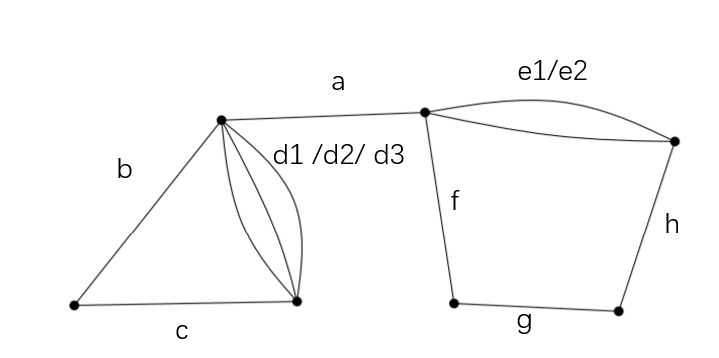
\includegraphics{3.ex.4.png}

\hypertarget{exercise-5}{%
\section{Exercise 5}\label{exercise-5}}

Let \(T\) be a minimum spanning tree of \(G\).

By exercise 2, we know that the connectivity of \(T_c\) is uniquely
determined.

The overall algorithm can be obtained by making a little modification to
the Kruskal's Algorithm.

\begin{enumerate}
\def\labelenumi{\arabic{enumi}.}
\item
  Sort all edges in the graph.
\item
  Traverse the sorted edges and group them together for the same edge
  weight \(w\).
\item
  Calculate the number of spanning trees with the weight of \(w\), and
  multiply the answer by this number. Then go to step 2.
\end{enumerate}

\end{document}
